\documentclass[11pt,letterpaper]{article}

% Page layout
\usepackage[margin=1in]{geometry}
\usepackage{setspace}
\onehalfspacing

% Typography and formatting
\usepackage{microtype}
\usepackage{titlesec}
\usepackage{enumitem}
\usepackage{booktabs}
\usepackage{longtable}
\usepackage{multirow}
\usepackage{array}
\usepackage{tabularx}
\usepackage{xcolor}
\usepackage{colortbl}

% Graphics and diagrams
\usepackage{tikz}
\usetikzlibrary{shapes.geometric, arrows.meta, positioning, fit, backgrounds, calc, decorations.pathreplacing, patterns, shadows}
\usepackage{pgfplots}
\pgfplotsset{compat=1.18}

% Code listings
\usepackage{listings}
\lstset{
    basicstyle=\ttfamily\small,
    breaklines=true,
    frame=single,
    backgroundcolor=\color{gray!10},
    keywordstyle=\color{blue},
    commentstyle=\color{green!50!black},
    stringstyle=\color{red!70!black},
}

% Math
\usepackage{amsmath,amssymb,amsthm}

% References and links
\usepackage[colorlinks=true,linkcolor=blue,citecolor=blue,urlcolor=blue]{hyperref}
\usepackage{cleveref}

% Bibliography
\usepackage[numbers,sort&compress]{natbib}

% Custom colors for diagrams
\definecolor{ucxblue}{RGB}{0,102,204}
\definecolor{ncclgreen}{RGB}{118,185,0}
\definecolor{cudaorange}{RGB}{255,153,0}
\definecolor{rdmared}{RGB}{204,0,0}
\definecolor{problemred}{RGB}{220,53,69}
\definecolor{solutiongreen}{RGB}{40,167,69}
\definecolor{layergray}{RGB}{240,240,240}
\definecolor{wfapurple}{RGB}{102,51,153}

% Custom theorem environments
\theoremstyle{definition}
\newtheorem{challenge}{Challenge}
\newtheorem{solution}{Proposed Solution}

% Title information
\title{
    \vspace{-1cm}
    \textbf{Adaptive RDMA Optimization for Distributed LLM Workloads} \\[0.5em]
    \large Update 7: Thesis Proposal --- A Unified Communication Framework Addressing\\Fragmentation Across NCCL, UCX, JACCL, and Emerging Standards
}

\author{
    Nathan Gopee \\
    \textit{MS Computer Science Candidate} \\
    SUNY New Paltz \\
    \texttt{gopeen1@newpaltz.edu} \\[1em]
    \small Advisors: Dr.\ Wafi Danesh \& Dr.\ Ashley Suchy
}

\date{February 2026}

\begin{document}

\maketitle

\begin{abstract}
\noindent
The distributed machine learning ecosystem suffers from fundamental architectural fragmentation across communication standards, creating compounding failures that block efficient training of large Mixture-of-Experts (MoE) models on consumer GPU clusters. This proposal presents a unified middleware framework that addresses seven critical blocking issues identified across NCCL, UCX, vLLM, Flash Attention, MLX/JACCL, and Exo: (1) cudaMallocAsync IPC incompatibility, (2) transport selection robustness failures, (3) container shared memory isolation, (4) cross-NUMA GPU latency regression, (5) RoCE reliability timeouts, (6) heterogeneous cluster build requirements, and (7) NCCL-UCX container integration. Our approach introduces a Weighted Finite Automaton (WFA) classifier for tensor-aware adaptive routing that operates above the transport layer, enabling intelligent differentiation of hot/warm/cold data paths without requiring modifications to existing RDMA stacks. We target 30--50\% reduction in Time-To-First-Token (TTFT) latency for distributed inference workloads on commodity hardware configurations including RTX 3090/5090 clusters connected via 10GbE with iWARP/RoCE capabilities.
\end{abstract}

\tableofcontents
\newpage

%=============================================================================
\section{Introduction and Problem Statement}
%=============================================================================

\subsection{The Multi-Standard Fragmentation Crisis}

Modern distributed machine learning infrastructure operates across incompatible communication layers that were designed independently for different hardware ecosystems. As shown in \Cref{fig:fragmentation-overview}, applications must navigate at least five distinct communication paths depending on hardware configuration, with no unified abstraction that preserves performance while enabling portability.

\begin{figure}[htbp]
\centering
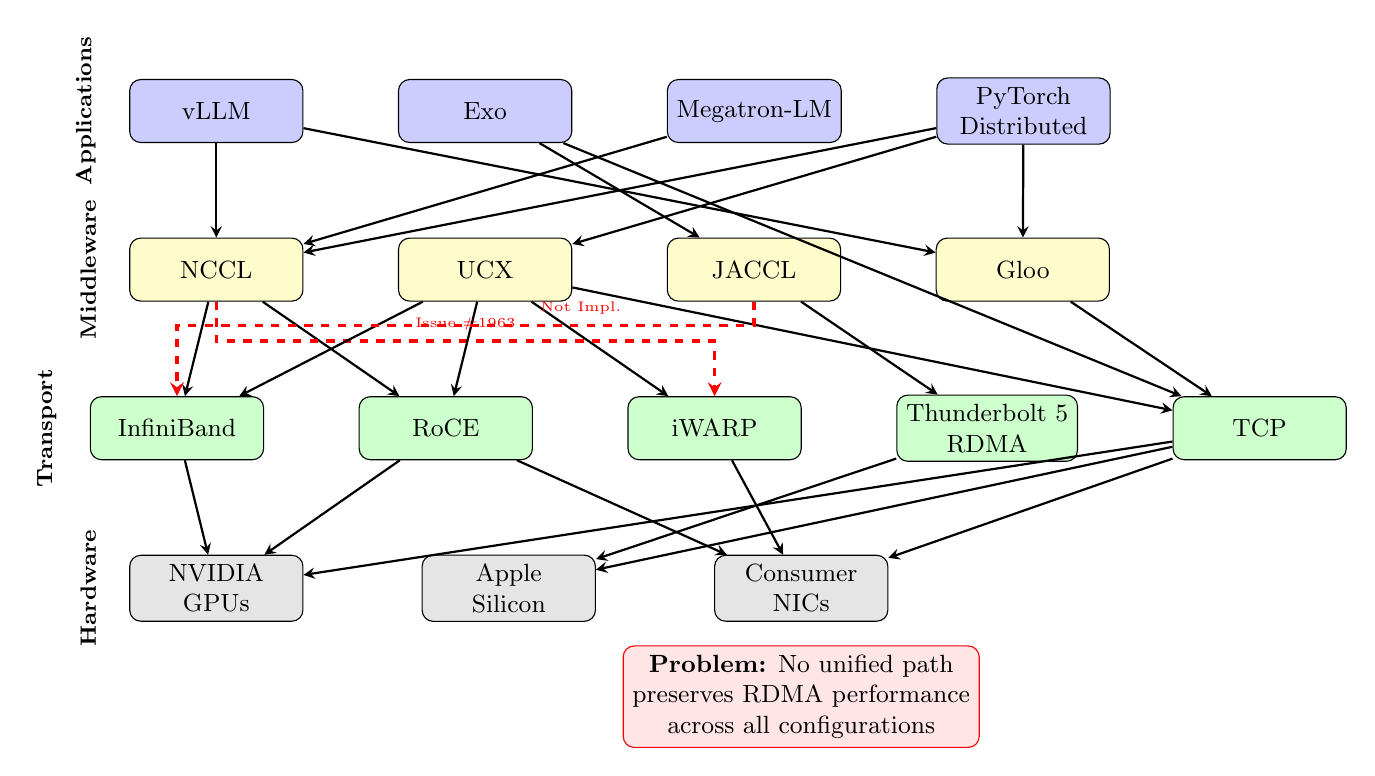
\begin{tikzpicture}[
    node distance=0.8cm and 1.2cm,
    box/.style={rectangle, draw, rounded corners, minimum width=2.2cm, minimum height=0.8cm, align=center, font=\small},
    app/.style={box, fill=blue!20},
    mid/.style={box, fill=yellow!20},
    trans/.style={box, fill=green!20},
    hw/.style={box, fill=gray!20},
    broken/.style={draw=red, very thick, dashed},
    arrow/.style={->, >=stealth, thick}
]

% Applications layer
\node[app] (vllm) {vLLM};
\node[app, right=of vllm] (exo) {Exo};
\node[app, right=of exo] (megatron) {Megatron-LM};
\node[app, right=of megatron] (pytorch) {PyTorch\\Distributed};

% Middleware layer
\node[mid, below=1.2cm of vllm] (nccl) {NCCL};
\node[mid, right=of nccl] (ucx) {UCX};
\node[mid, right=of ucx] (jaccl) {JACCL};
\node[mid, right=of jaccl] (gloo) {Gloo};

% Transport layer
\node[trans, below=1.2cm of nccl, xshift=-0.5cm] (ib) {InfiniBand};
\node[trans, right=of ib] (roce) {RoCE};
\node[trans, right=of roce] (iwarp) {iWARP};
\node[trans, right=of iwarp] (tb5) {Thunderbolt 5\\RDMA};
\node[trans, right=of tb5] (tcp) {TCP};

% Hardware layer
\node[hw, below=1.2cm of ib, xshift=0.5cm] (nvidia) {NVIDIA\\GPUs};
\node[hw, right=1.5cm of nvidia] (apple) {Apple\\Silicon};
\node[hw, right=1.5cm of apple] (consumer) {Consumer\\NICs};

% Arrows from apps to middleware
\draw[arrow] (vllm) -- (nccl);
\draw[arrow] (vllm) -- (gloo);
\draw[arrow] (exo) -- (jaccl);
\draw[arrow] (exo) -- (tcp);
\draw[arrow] (megatron) -- (nccl);
\draw[arrow] (pytorch) -- (nccl);
\draw[arrow] (pytorch) -- (gloo);
\draw[arrow] (pytorch) -- (ucx);

% Arrows from middleware to transport
\draw[arrow] (nccl) -- (ib);
\draw[arrow] (nccl) -- (roce);
\draw[arrow, broken] (nccl.south) -- ++(0,-0.5) -| (iwarp) node[pos=0.25, above, font=\tiny\color{red}] {Issue \#1963};
\draw[arrow] (ucx) -- (ib);
\draw[arrow] (ucx) -- (roce);
\draw[arrow] (ucx) -- (iwarp);
\draw[arrow] (ucx) -- (tcp);
\draw[arrow] (jaccl) -- (tb5);
\draw[arrow, broken] (jaccl.south) -- ++(0,-0.3) -| (ib) node[pos=0.15, above, font=\tiny\color{red}] {Not Impl.};
\draw[arrow] (gloo) -- (tcp);

% Arrows from transport to hardware
\draw[arrow] (ib) -- (nvidia);
\draw[arrow] (roce) -- (nvidia);
\draw[arrow] (roce) -- (consumer);
\draw[arrow] (iwarp) -- (consumer);
\draw[arrow] (tb5) -- (apple);
\draw[arrow] (tcp) -- (nvidia);
\draw[arrow] (tcp) -- (apple);
\draw[arrow] (tcp) -- (consumer);

% Layer labels
\node[left=0.3cm of vllm, font=\footnotesize\bfseries, rotate=90, anchor=south] {Applications};
\node[left=0.3cm of nccl, font=\footnotesize\bfseries, rotate=90, anchor=south] {Middleware};
\node[left=0.3cm of ib, font=\footnotesize\bfseries, rotate=90, anchor=south] {Transport};
\node[left=0.3cm of nvidia, font=\footnotesize\bfseries, rotate=90, anchor=south] {Hardware};

% Problem callout
\node[draw=red, fill=red!10, rounded corners, font=\small, align=center, below=0.3cm of consumer] (problem) {
    \textbf{Problem:} No unified path\\preserves RDMA performance\\across all configurations
};

\end{tikzpicture}
\caption{Current fragmentation in distributed ML communication stacks. Dashed red lines indicate broken or unimplemented paths identified through GitHub issue analysis.}
\label{fig:fragmentation-overview}
\end{figure}

\subsection{Research Objectives}

This thesis proposes to:

\begin{enumerate}[label=\textbf{O\arabic*.}]
    \item Design and implement a unified middleware layer that abstracts transport-specific details while preserving RDMA performance characteristics
    \item Develop a Weighted Finite Automaton (WFA) classifier that categorizes tensor access patterns as hot/warm/cold for differential routing
    \item Address the seven critical blocking issues preventing UCX adoption as a unified communication standard
    \item Validate the approach through both simulation (UET-HTSIM) and real hardware deployment (RTX 3090/5090 cluster with 10GbE iWARP)
    \item Demonstrate applicability to MoE model training (Granite 4/Mamba 2 architectures) for RISC-V assembly generation
\end{enumerate}

%=============================================================================
\section{Critical Issues Analysis}
%=============================================================================

This section details the seven blocking issues identified through comprehensive GitHub issue analysis across NCCL, UCX, vLLM, Flash Attention, MLX/JACCL, and Exo repositories.

%-----------------------------------------------------------------------------
\subsection{Issue 1: cudaMallocAsync IPC Incompatibility (UCX \#7110)}
%-----------------------------------------------------------------------------

\begin{challenge}
Modern PyTorch memory pools use \texttt{cudaMallocAsync} for efficient GPU memory allocation, but these allocations do not support \texttt{cuIpcGetMemHandle}, breaking GPU RDMA for inter-process communication.
\end{challenge}

\begin{figure}[htbp]
\centering
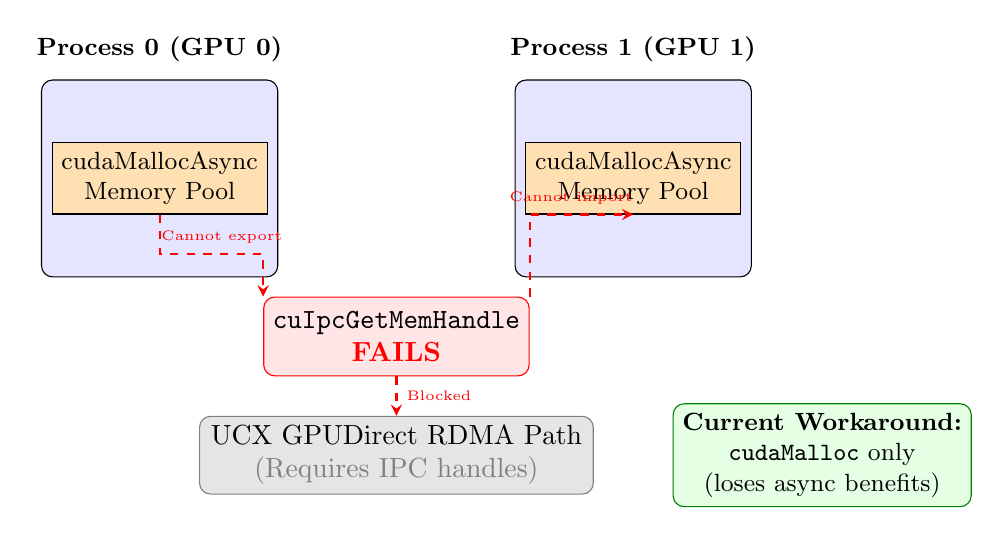
\begin{tikzpicture}[
    node distance=0.6cm and 1.5cm,
    process/.style={rectangle, draw, rounded corners, minimum width=3cm, minimum height=2.5cm, align=center},
    mem/.style={rectangle, draw, fill=cudaorange!30, minimum width=2.2cm, minimum height=0.6cm, align=center, font=\small},
    arrow/.style={->, >=stealth, thick},
    broken/.style={->, >=stealth, thick, dashed, red},
    label/.style={font=\footnotesize}
]

% Process 0
\node[process, fill=blue!10] (p0) {};
\node[above=0.1cm of p0.north, font=\small\bfseries] {Process 0 (GPU 0)};
\node[mem] (cuda0) at (p0.center) {cudaMallocAsync\\Memory Pool};

% Process 1
\node[process, fill=blue!10, right=3cm of p0] (p1) {};
\node[above=0.1cm of p1.north, font=\small\bfseries] {Process 1 (GPU 1)};
\node[mem] (cuda1) at (p1.center) {cudaMallocAsync\\Memory Pool};

% IPC attempt
\node[draw=red, fill=red!10, rounded corners, minimum width=2.5cm, minimum height=1cm, below=1.5cm of $(p0)!0.5!(p1)$, align=center] (ipc) {
    \texttt{cuIpcGetMemHandle}\\
    \textcolor{red}{\textbf{FAILS}}
};

% Arrows
\draw[broken] (cuda0.south) -- ++(0,-0.5) -| (ipc.north west) node[pos=0.3, above, font=\tiny] {Cannot export};
\draw[broken] (ipc.north east) |- (cuda1.south) node[pos=0.7, above, font=\tiny] {Cannot import};

% UCX RDMA path
\node[draw=gray, fill=gray!20, rounded corners, below=0.5cm of ipc, minimum width=5cm, align=center] (ucx) {
    UCX GPUDirect RDMA Path\\
    \textcolor{gray}{(Requires IPC handles)}
};

\draw[broken] (ipc) -- (ucx) node[midway, right, font=\tiny\color{red}] {Blocked};

% Current workaround
\node[draw=green!50!black, fill=green!10, rounded corners, right=1cm of ucx, minimum width=3cm, align=center, font=\small] (workaround) {
    \textbf{Current Workaround:}\\
    \texttt{cudaMalloc} only\\
    (loses async benefits)
};

\end{tikzpicture}
\caption{cudaMallocAsync IPC incompatibility blocks modern PyTorch memory pools from using UCX RDMA.}
\label{fig:cuda-ipc}
\end{figure}

\begin{solution}
We propose a \textbf{Memory Pool Proxy Layer} that:
\begin{enumerate}
    \item Intercepts tensor allocations before they reach PyTorch's memory allocator
    \item Maintains a shadow pool of IPC-exportable memory regions pre-registered with UCX
    \item Performs transparent copy-on-RDMA-request for async-allocated tensors that require inter-process transfer
    \item Caches frequently-transferred tensors in the IPC-compatible pool based on WFA classifier predictions
\end{enumerate}
\end{solution}

%-----------------------------------------------------------------------------
\subsection{Issue 2: Transport Selection Robustness (UCX \#9908)}
%-----------------------------------------------------------------------------

\begin{challenge}
UCX fails when \texttt{UCX\_TLS} is set to any transport other than ``rc'' (Reliable Connection) for multi-node training, limiting transport flexibility and preventing automatic fallback.
\end{challenge}

\begin{figure}[htbp]
\centering
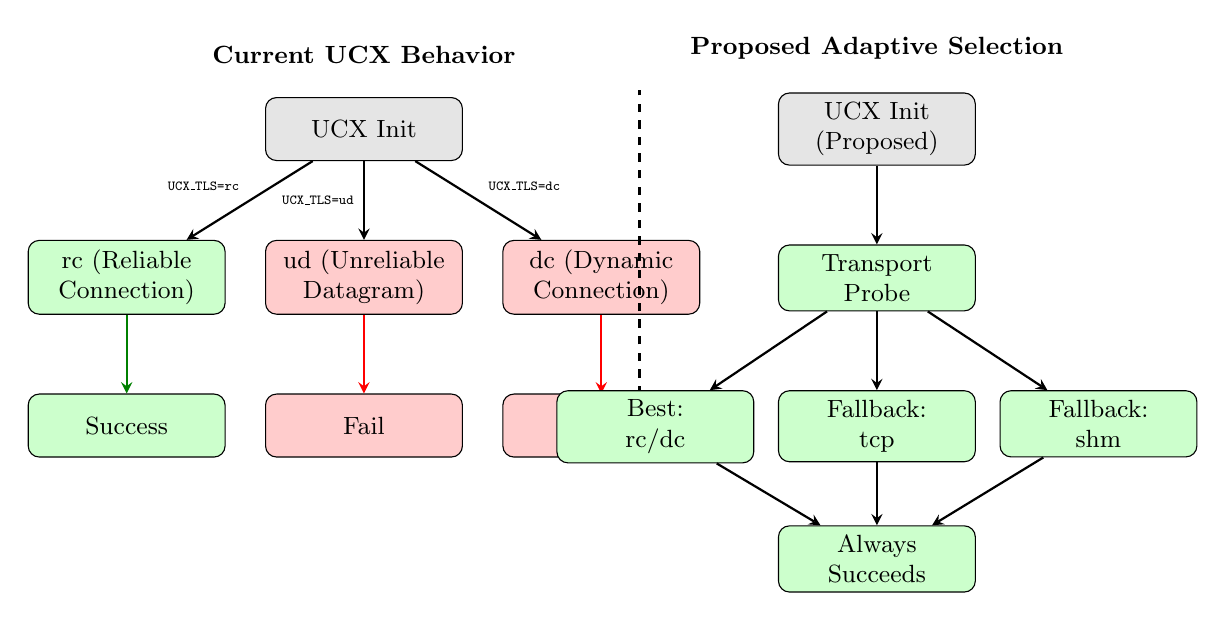
\begin{tikzpicture}[
    node distance=0.5cm,
    state/.style={rectangle, draw, rounded corners, minimum width=2.5cm, minimum height=0.8cm, align=center, font=\small},
    good/.style={state, fill=green!20},
    bad/.style={state, fill=red!20},
    neutral/.style={state, fill=gray!20},
    arrow/.style={->, >=stealth, thick},
    label/.style={font=\footnotesize}
]

% Current behavior
\node[neutral] (start) {UCX Init};
\node[good, below left=1cm and 0.5cm of start] (rc) {rc (Reliable\\Connection)};
\node[bad, below=1cm of start] (ud) {ud (Unreliable\\Datagram)};
\node[bad, below right=1cm and 0.5cm of start] (dc) {dc (Dynamic\\Connection)};

\node[good, below=1cm of rc] (rcok) {Success};
\node[bad, below=1cm of ud] (udfail) {Fail};
\node[bad, below=1cm of dc] (dcfail) {Fail};

\draw[arrow] (start) -- node[above left, font=\tiny] {\texttt{UCX\_TLS=rc}} (rc);
\draw[arrow] (start) -- node[left, font=\tiny] {\texttt{UCX\_TLS=ud}} (ud);
\draw[arrow] (start) -- node[above right, font=\tiny] {\texttt{UCX\_TLS=dc}} (dc);

\draw[arrow, green!50!black] (rc) -- (rcok);
\draw[arrow, red] (ud) -- (udfail);
\draw[arrow, red] (dc) -- (dcfail);

% Divider
\draw[dashed, thick] (3.5,-4) -- (3.5,0.5);

% Proposed behavior
\node[neutral, right=4cm of start] (start2) {UCX Init\\(Proposed)};
\node[good, below=1cm of start2] (probe) {Transport\\Probe};
\node[good, below left=1cm and 0.3cm of probe] (t1) {Best:\\rc/dc};
\node[good, below=1cm of probe] (t2) {Fallback:\\tcp};
\node[good, below right=1cm and 0.3cm of probe] (t3) {Fallback:\\shm};

\node[good, below=0.8cm of t2] (success) {Always\\Succeeds};

\draw[arrow] (start2) -- (probe);
\draw[arrow] (probe) -- (t1);
\draw[arrow] (probe) -- (t2);
\draw[arrow] (probe) -- (t3);
\draw[arrow] (t1) -- (success);
\draw[arrow] (t2) -- (success);
\draw[arrow] (t3) -- (success);

% Labels
\node[above=0.3cm of start, font=\small\bfseries] {Current UCX Behavior};
\node[above=0.3cm of start2, font=\small\bfseries] {Proposed Adaptive Selection};

\end{tikzpicture}
\caption{Transport selection failure modes in current UCX vs.\ proposed adaptive selection with graceful fallback.}
\label{fig:transport-selection}
\end{figure}

\begin{solution}
Implement a \textbf{Transport Capability Negotiation Protocol} that:
\begin{enumerate}
    \item Probes available transports at connection establishment time
    \item Maintains a priority list: \{dc, rc, ud, tcp, shm\} with dynamic reordering based on observed performance
    \item Automatically falls back to lower-priority transports on failure
    \item Exposes transport selection decisions to the WFA classifier for learning
\end{enumerate}
\end{solution}

%-----------------------------------------------------------------------------
\subsection{Issue 3: Container Shared Memory Isolation (UCX \#10055)}
%-----------------------------------------------------------------------------

\begin{challenge}
NCCL all-reduce operations fail with ``Child failed to attach to shmseg'' errors when running in containers on the same server, even with \texttt{--ipc=host} Docker flags.
\end{challenge}

\begin{figure}[htbp]
\centering
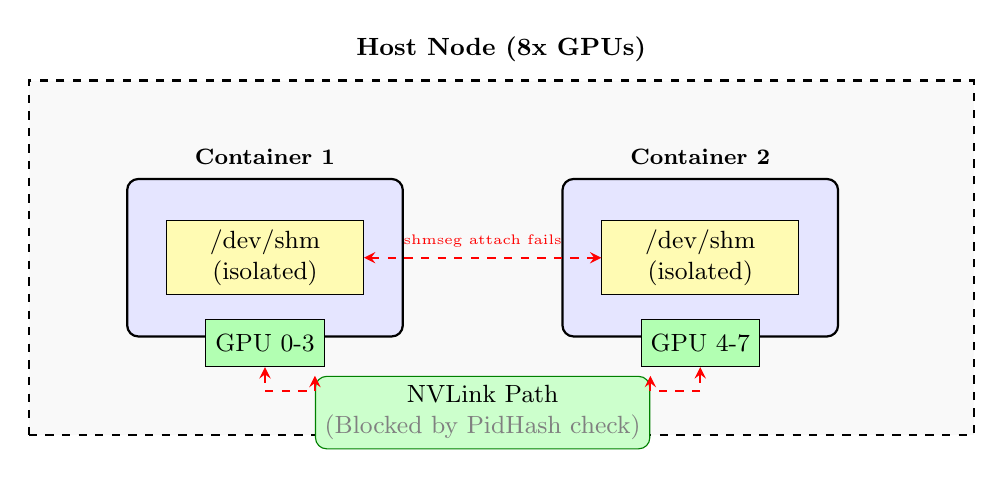
\begin{tikzpicture}[
    node distance=0.8cm,
    container/.style={rectangle, draw, thick, rounded corners, minimum width=3.5cm, minimum height=2cm, fill=blue!10},
    shm/.style={rectangle, draw, fill=yellow!30, minimum width=2.5cm, minimum height=0.6cm, align=center, font=\small},
    gpu/.style={rectangle, draw, fill=green!30, minimum width=1.5cm, minimum height=0.6cm, align=center, font=\small},
    host/.style={rectangle, draw, dashed, thick, minimum width=12cm, minimum height=4.5cm},
    arrow/.style={->, >=stealth, thick},
    broken/.style={<->, >=stealth, thick, dashed, red}
]

% Host boundary
\node[host, fill=gray!5] (host) {};
\node[above=0.1cm of host.north, font=\small\bfseries] {Host Node (8x GPUs)};

% Container 1
\node[container] (c1) at (-3, 0) {};
\node[above=0.05cm of c1.north, font=\footnotesize\bfseries] {Container 1};
\node[shm] (shm1) at (c1.center) {/dev/shm\\(isolated)};
\node[gpu, below=0.3cm of shm1] (gpu1) {GPU 0-3};

% Container 2
\node[container, right=2cm of c1] (c2) {};
\node[above=0.05cm of c2.north, font=\footnotesize\bfseries] {Container 2};
\node[shm] (shm2) at (c2.center) {/dev/shm\\(isolated)};
\node[gpu, below=0.3cm of shm2] (gpu2) {GPU 4-7};

% NCCL P2P attempt
\draw[broken] (shm1.east) -- (shm2.west) node[midway, above, font=\tiny\color{red}] {shmseg attach fails};

% NVLink (works)
\node[draw=green!50!black, fill=green!20, rounded corners, below=1.5cm of $(c1)!0.5!(c2)$, minimum width=4cm, align=center, font=\small] (nvlink) {
    NVLink Path\\
    \textcolor{gray}{(Blocked by PidHash check)}
};

\draw[broken] (gpu1.south) -- ++(0,-0.3) -| (nvlink.north west);
\draw[broken] (gpu2.south) -- ++(0,-0.3) -| (nvlink.north east);

\end{tikzpicture}
\caption{Container isolation prevents shared memory IPC between NCCL processes, even when GPUs are physically connected via NVLink.}
\label{fig:container-shm}
\end{figure}

\begin{solution}
Our middleware introduces a \textbf{Container-Aware Communication Broker}:
\begin{enumerate}
    \item Detects container boundaries via cgroup inspection
    \item Establishes a host-level coordinator process with access to unified \texttt{/dev/shm}
    \item Routes intra-node communication through the coordinator when direct shm attachment fails
    \item Falls back to NVLink P2P with modified PidHash validation (requires \texttt{NCCL\_HOSTID=0.0.0.0})
\end{enumerate}
\end{solution}

%-----------------------------------------------------------------------------
\subsection{Issue 4: Cross-NUMA GPU Latency Regression (UCX \#3249)}
%-----------------------------------------------------------------------------

\begin{challenge}
GPU-to-GPU communication experiences 10$\times$ latency degradation for messages larger than 262KB when GPUs reside in different NUMA domains.
\end{challenge}

\begin{figure}[htbp]
\centering
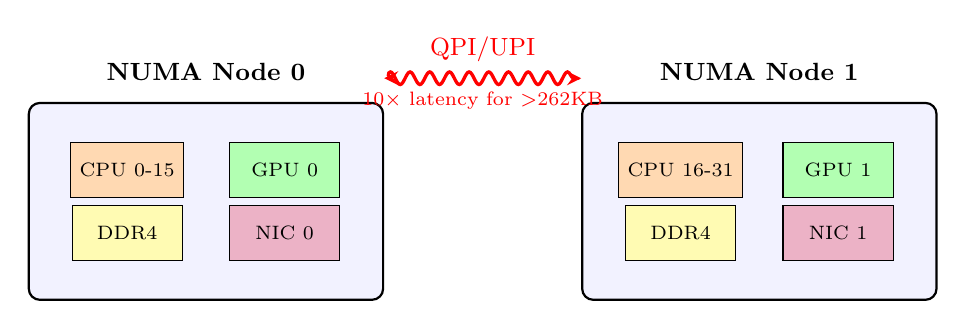
\begin{tikzpicture}[
    node distance=0.5cm,
    numa/.style={rectangle, draw, thick, rounded corners, minimum width=4.5cm, minimum height=2.5cm, fill=blue!5},
    cpu/.style={rectangle, draw, fill=orange!30, minimum width=1.4cm, minimum height=0.7cm, align=center, font=\scriptsize},
    gpu/.style={rectangle, draw, fill=green!30, minimum width=1.4cm, minimum height=0.7cm, align=center, font=\scriptsize},
    mem/.style={rectangle, draw, fill=yellow!30, minimum width=1.4cm, minimum height=0.7cm, align=center, font=\scriptsize},
    nic/.style={rectangle, draw, fill=purple!30, minimum width=1.4cm, minimum height=0.7cm, align=center, font=\scriptsize},
    arrow/.style={->, >=stealth, thick},
    slow/.style={<->, >=stealth, very thick, red, decorate, decoration={snake, amplitude=0.8mm, segment length=2.5mm}}
]

% NUMA 0
\node[numa] (numa0) at (0,0) {};
\node[above=0.15cm of numa0.north, font=\small\bfseries] {NUMA Node 0};
\node[cpu] (cpu0) at (-1, 0.4) {CPU 0-15};
\node[gpu] (gpu0) at (1, 0.4) {GPU 0};
\node[mem] (mem0) at (-1, -0.4) {DDR4};
\node[nic] (nic0) at (1, -0.4) {NIC 0};

% NUMA 1
\node[numa, right=2.5cm of numa0] (numa1) {};
\node[above=0.15cm of numa1.north, font=\small\bfseries] {NUMA Node 1};
\node[cpu] (cpu1) at ($(numa1.center)+(-1, 0.4)$) {CPU 16-31};
\node[gpu] (gpu1) at ($(numa1.center)+(1, 0.4)$) {GPU 1};
\node[mem] (mem1) at ($(numa1.center)+(-1, -0.4)$) {DDR4};
\node[nic] (nic1) at ($(numa1.center)+(1, -0.4)$) {NIC 1};

% QPI interconnect - positioned above the nodes
\draw[slow] ($(numa0.north east)+(0,0.3)$) -- ($(numa1.north west)+(0,0.3)$) node[midway, above=2pt, font=\small] {QPI/UPI};
\node[below=0.05cm of $(numa0.north east)!0.5!(numa1.north west)$, yshift=0.3cm, font=\scriptsize\color{red}] {10$\times$ latency for $>$262KB};

\end{tikzpicture}

\vspace{0.5cm}

% Separate bar chart below
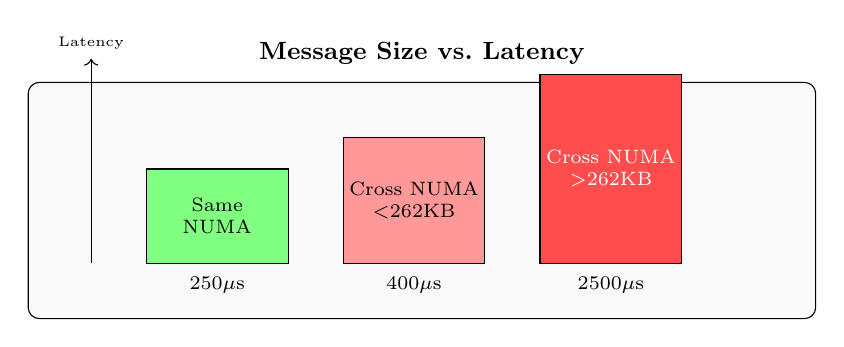
\begin{tikzpicture}
\node[draw, fill=gray!5, rounded corners, minimum width=10cm, minimum height=3cm] (chart) {};
\node[above=0.1cm of chart.north, font=\small\bfseries] {Message Size vs.\ Latency};

% Bar chart with proper spacing
\draw[fill=green!50] (-3.5,-0.8) rectangle ++(1.8,1.2);
\node[font=\scriptsize, align=center] at (-2.6, -0.2) {Same\\NUMA};
\node[font=\scriptsize, below] at (-2.6, -0.85) {250$\mu$s};

\draw[fill=red!40] (-1,-0.8) rectangle ++(1.8,1.6);
\node[font=\scriptsize, align=center] at (-0.1, 0) {Cross NUMA\\$<$262KB};
\node[font=\scriptsize, below] at (-0.1, -0.85) {400$\mu$s};

\draw[fill=red!70] (1.5,-0.8) rectangle ++(1.8,2.4);
\node[font=\scriptsize, align=center, text=white] at (2.4, 0.4) {Cross NUMA\\$>$262KB};
\node[font=\scriptsize, below] at (2.4, -0.85) {2500$\mu$s};

% Y-axis indicator
\draw[->] (-4.2,-0.8) -- (-4.2,1.8) node[above, font=\tiny] {Latency};

\end{tikzpicture}
\caption{Cross-NUMA GPU communication latency explodes for larger message sizes due to memory controller contention.}
\label{fig:numa-latency}
\end{figure}

\begin{solution}
The WFA classifier integrates \textbf{NUMA-Aware Tensor Placement}:
\begin{enumerate}
    \item Queries sysfs topology to determine GPU-NIC-CPU NUMA relationships
    \item Fragments messages $>$256KB crossing NUMA boundaries into pipelined chunks
    \item Prioritizes NUMA-local bounce buffers for staging cross-domain transfers
    \item Preemptively migrates frequently-accessed tensors to NUMA-optimal locations
\end{enumerate}
\end{solution}

%-----------------------------------------------------------------------------
\subsection{Issue 5: RoCE Reliability Timeouts (UCX \#6000)}
%-----------------------------------------------------------------------------

\begin{challenge}
Multi-node RoCE deployments crash after approximately 90 seconds with ``Transport retry count exceeded on mlx5/RoCE'' errors, making long-running training jobs impossible.
\end{challenge}

\begin{figure}[htbp]
\centering
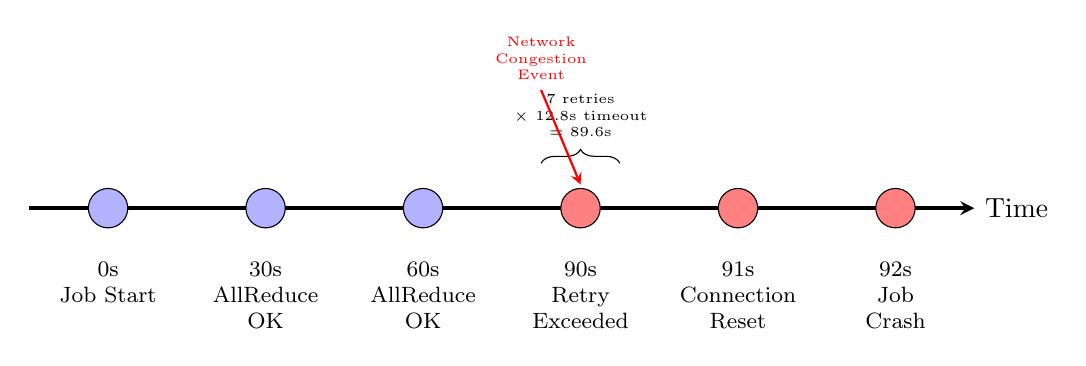
\begin{tikzpicture}[
    node distance=1cm,
    timeline/.style={->, >=stealth, very thick},
    event/.style={circle, draw, fill=blue!30, minimum size=0.5cm},
    fail/.style={circle, draw, fill=red!50, minimum size=0.5cm},
    label/.style={font=\footnotesize, align=center}
]

% Timeline
\draw[timeline] (0,0) -- (12,0) node[right] {Time};

% Events
\node[event] (e1) at (1,0) {};
\node[label, below=0.3cm of e1] {0s\\Job Start};

\node[event] (e2) at (3,0) {};
\node[label, below=0.3cm of e2] {30s\\AllReduce\\OK};

\node[event] (e3) at (5,0) {};
\node[label, below=0.3cm of e3] {60s\\AllReduce\\OK};

\node[fail] (e4) at (7,0) {};
\node[label, below=0.3cm of e4] {90s\\Retry\\Exceeded};

\node[fail] (e5) at (9,0) {};
\node[label, below=0.3cm of e5] {91s\\Connection\\Reset};

\node[fail] (e6) at (11,0) {};
\node[label, below=0.3cm of e6] {92s\\Job\\Crash};

% RoCE retry behavior
\draw[decorate, decoration={brace, amplitude=5pt, raise=2pt}] (6.5,0.5) -- (7.5,0.5) node[midway, above=8pt, font=\tiny, align=center] {7 retries\\$\times$ 12.8s timeout\\= 89.6s};

% Congestion event
\draw[->, >=stealth, thick, red] (6.5, 1.5) -- (7, 0.3) node[pos=0, above, font=\tiny, align=center] {Network\\Congestion\\Event};

\end{tikzpicture}
\caption{RoCE retry timeout accumulation leads to catastrophic failure after $\sim$90 seconds of congestion.}
\label{fig:roce-timeout}
\end{figure}

\begin{solution}
Implement \textbf{Proactive Congestion Detection and Path Switching}:
\begin{enumerate}
    \item Monitor RTT variance and ECN marks to detect congestion before retry exhaustion
    \item Maintain backup QP connections that can be hot-swapped on primary path degradation
    \item Integrate with WFA classifier to preemptively route sensitive tensors away from congested paths
    \item Implement application-level ACK coalescing to reduce retry pressure
\end{enumerate}
\end{solution}

%-----------------------------------------------------------------------------
\subsection{Issue 6: Heterogeneous Cluster Builds (UCX \#10273)}
%-----------------------------------------------------------------------------

\begin{challenge}
UCX cannot be built as a single binary that works across both GPU-enabled and CPU-only nodes, requiring separate builds and complicating deployment.
\end{challenge}

\begin{figure}[htbp]
\centering
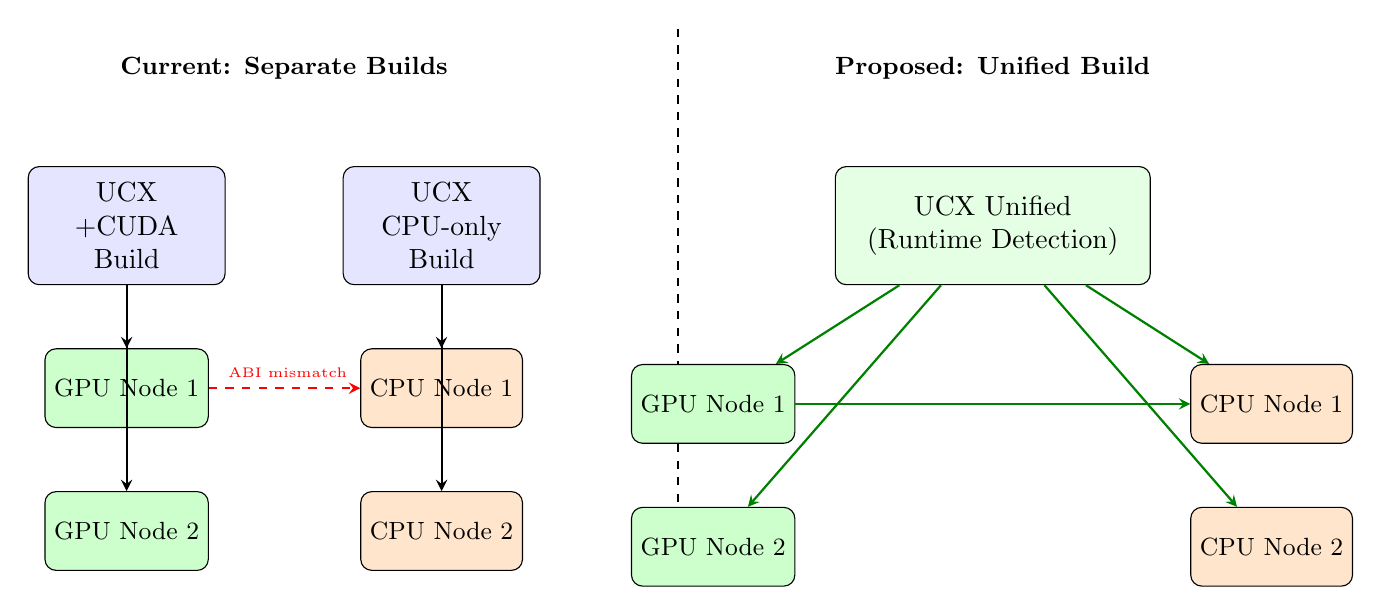
\begin{tikzpicture}[
    node distance=0.8cm,
    build/.style={rectangle, draw, rounded corners, minimum width=2.5cm, minimum height=1.5cm, align=center, fill=blue!10},
    node/.style={rectangle, draw, rounded corners, minimum width=2cm, minimum height=1cm, align=center, font=\small},
    gpunode/.style={node, fill=green!20},
    cpunode/.style={node, fill=orange!20},
    arrow/.style={->, >=stealth, thick},
    broken/.style={->, >=stealth, thick, dashed, red}
]

% Current approach
\node[font=\small\bfseries] (current) at (0, 2) {Current: Separate Builds};

\node[build] (gpubuild) at (-2, 0) {UCX\\+CUDA\\Build};
\node[build] (cpubuild) at (2, 0) {UCX\\CPU-only\\Build};

\node[gpunode, below=of gpubuild] (gpu1) {GPU Node 1};
\node[gpunode, below=of gpu1] (gpu2) {GPU Node 2};
\node[cpunode, below=of cpubuild] (cpu1) {CPU Node 1};
\node[cpunode, below=of cpu1] (cpu2) {CPU Node 2};

\draw[arrow] (gpubuild) -- (gpu1);
\draw[arrow] (gpubuild) -- (gpu2);
\draw[arrow] (cpubuild) -- (cpu1);
\draw[arrow] (cpubuild) -- (cpu2);

\draw[broken] (gpu1.east) -- ++(1,0) |- (cpu1.west) node[pos=0.25, above, font=\tiny\color{red}] {ABI mismatch};

% Divider
\draw[dashed, thick] (5, 2.5) -- (5, -4);

% Proposed approach
\node[font=\small\bfseries] (proposed) at (9, 2) {Proposed: Unified Build};

\node[build, minimum width=4cm, fill=green!10] (unified) at (9, 0) {UCX Unified\\(Runtime Detection)};

\node[gpunode, below left=1cm and 0.5cm of unified] (gpu1p) {GPU Node 1};
\node[gpunode, below=of gpu1p] (gpu2p) {GPU Node 2};
\node[cpunode, below right=1cm and 0.5cm of unified] (cpu1p) {CPU Node 1};
\node[cpunode, below=of cpu1p] (cpu2p) {CPU Node 2};

\draw[arrow, green!50!black] (unified) -- (gpu1p);
\draw[arrow, green!50!black] (unified) -- (gpu2p);
\draw[arrow, green!50!black] (unified) -- (cpu1p);
\draw[arrow, green!50!black] (unified) -- (cpu2p);

\draw[arrow, green!50!black] (gpu1p.east) -- ++(0.5,0) |- (cpu1p.west);

\end{tikzpicture}
\caption{Heterogeneous cluster deployment requires separate UCX builds in current approach vs.\ proposed unified runtime-detection build.}
\label{fig:heterogeneous}
\end{figure}

\begin{solution}
Our middleware provides a \textbf{Capability Abstraction Layer}:
\begin{enumerate}
    \item Wraps UCX initialization with runtime CUDA availability detection
    \item Gracefully degrades GPU-specific features when CUDA libraries are unavailable
    \item Maintains ABI compatibility across node types through stable interface versioning
    \item Enables mixed CPU/GPU deployments for MoE expert placement optimization
\end{enumerate}
\end{solution}

%-----------------------------------------------------------------------------
\subsection{Issue 7: NCCL-UCX Container Integration (UCX \#10055)}
%-----------------------------------------------------------------------------

\begin{challenge}
Running NCCL with UCX as the network backend in containerized environments produces ``TL\_SHM ERROR'' failures due to shared memory namespace isolation.
\end{challenge}

\begin{figure}[htbp]
\centering
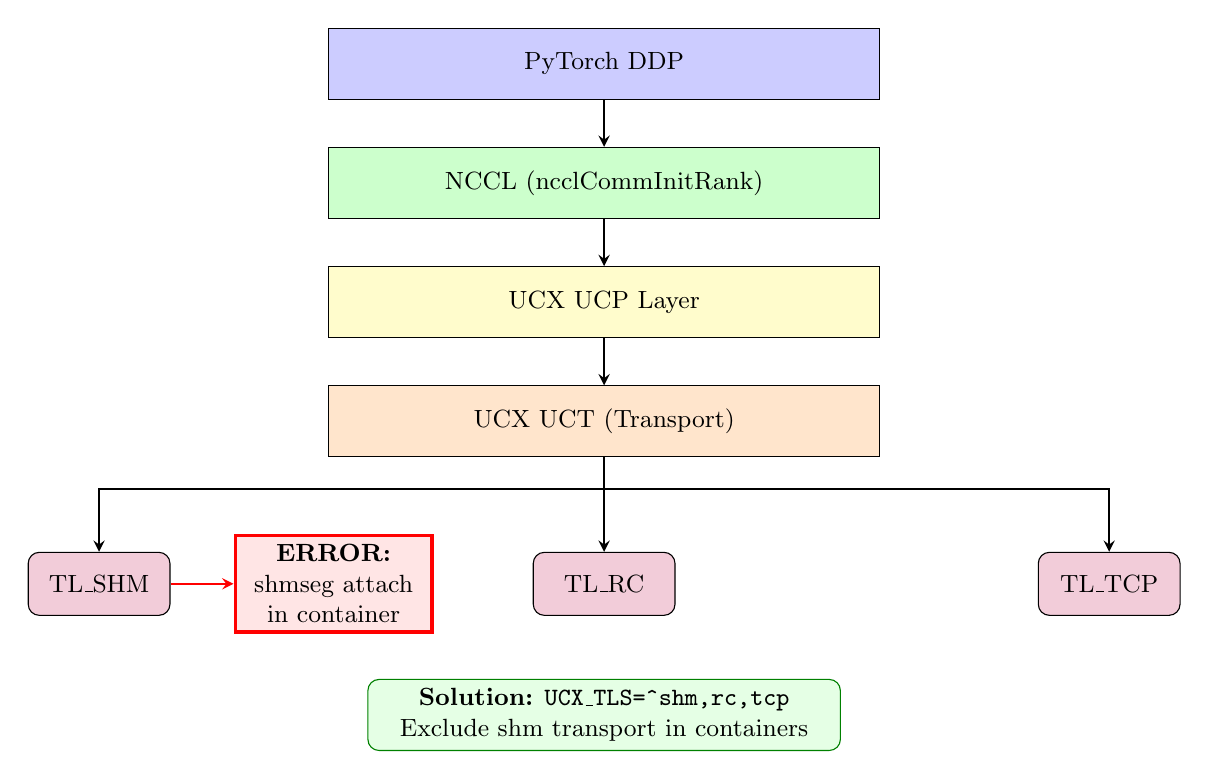
\begin{tikzpicture}[
    node distance=0.8cm,
    layer/.style={rectangle, draw, minimum width=7cm, minimum height=0.9cm, align=center, font=\small},
    transport/.style={rectangle, draw, rounded corners, minimum width=1.8cm, minimum height=0.8cm, align=center, font=\small},
    app/.style={layer, fill=blue!20},
    nccl/.style={layer, fill=green!20},
    ucx/.style={layer, fill=yellow!20},
    trans/.style={layer, fill=orange!20},
    error/.style={draw=red, very thick, fill=red!10},
    arrow/.style={->, >=stealth, thick}
]

% Stack - vertical layout with more spacing
\node[app] (pytorch) {PyTorch DDP};
\node[nccl, below=0.6cm of pytorch] (nccl) {NCCL (ncclCommInitRank)};
\node[ucx, below=0.6cm of nccl] (ucp) {UCX UCP Layer};
\node[trans, below=0.6cm of ucp] (uct) {UCX UCT (Transport)};

% Transport options - spread out horizontally
\node[transport, fill=purple!20, below left=1.2cm and 2cm of uct] (shm) {TL\_SHM};
\node[transport, fill=purple!20, below=1.2cm of uct] (rc) {TL\_RC};
\node[transport, fill=purple!20, below right=1.2cm and 2cm of uct] (tcp) {TL\_TCP};

% Arrows from stack
\draw[arrow] (pytorch) -- (nccl);
\draw[arrow] (nccl) -- (ucp);
\draw[arrow] (ucp) -- (uct);
\draw[arrow] (uct.south) -- ++(0,-0.4) -| (shm.north);
\draw[arrow] (uct) -- (rc);
\draw[arrow] (uct.south) -- ++(0,-0.4) -| (tcp.north);

% Error callout - positioned to the right of TL_SHM, not overlapping
\node[error, right=0.8cm of shm, minimum width=2.5cm, minimum height=1.2cm, align=center, font=\small] (err) {
    \textbf{ERROR:}\\
    shmseg attach\\
    in container
};
\draw[arrow, red, thick] (shm.east) -- (err.west);

% Solution box - below everything
\node[draw=green!50!black, fill=green!10, rounded corners, below=0.8cm of rc, minimum width=6cm, align=center, font=\small] (solution) {
    \textbf{Solution:} \texttt{UCX\_TLS=\textasciicircum shm,rc,tcp}\\
    Exclude shm transport in containers
};

\end{tikzpicture}
\caption{NCCL-over-UCX fails in containers when UCX attempts to use shared memory transport.}
\label{fig:nccl-ucx}
\end{figure}

\begin{solution}
Automatic \textbf{Container Environment Detection and Transport Filtering}:
\begin{enumerate}
    \item Detect containerization via \texttt{/proc/1/cgroup} inspection
    \item Automatically exclude shm transport when running in containers
    \item Provide environment variable presets for common container runtimes (Docker, Kubernetes, Singularity)
    \item Integrate fix into middleware initialization to eliminate manual configuration
\end{enumerate}
\end{solution}

%=============================================================================
\section{Proposed Architecture}
%=============================================================================

\subsection{System Overview}

\Cref{fig:system-architecture} presents the complete system architecture, showing how the proposed middleware layer integrates with existing communication stacks.

\begin{figure}[htbp]
\centering
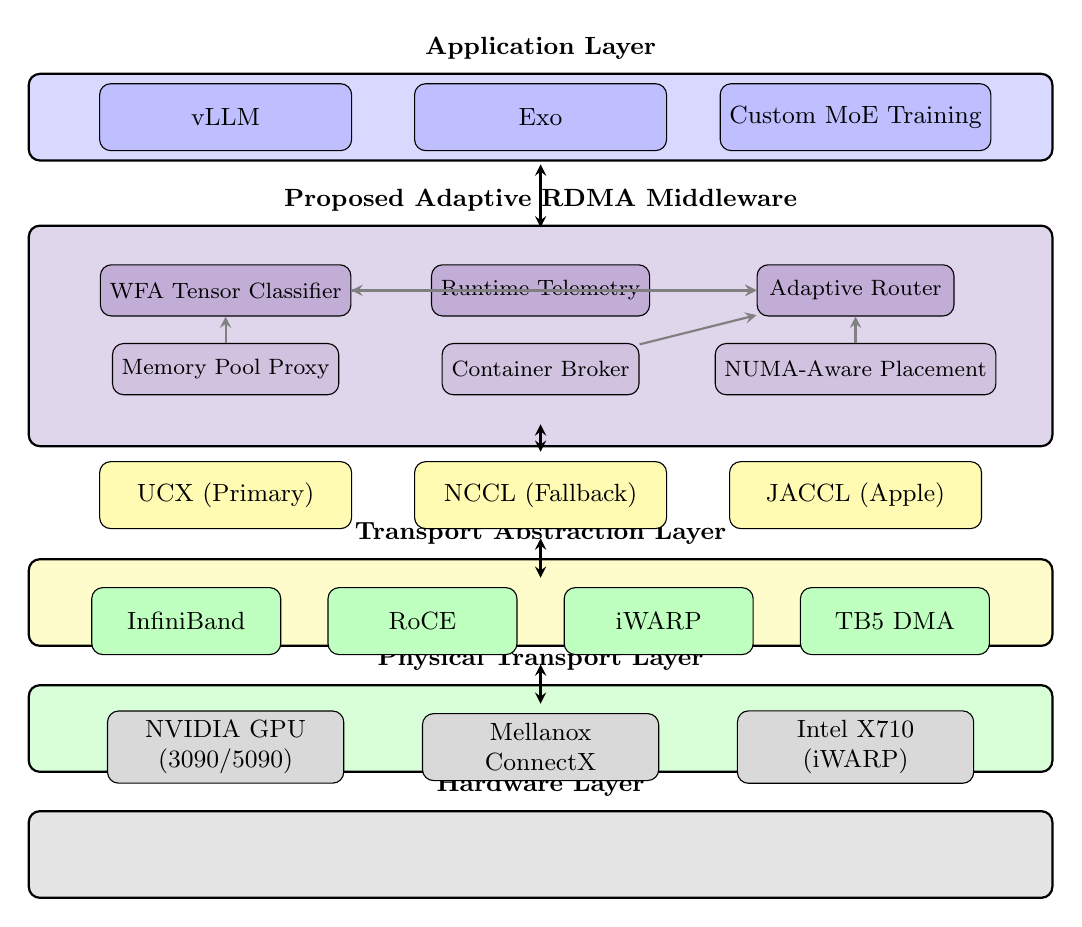
\begin{tikzpicture}[
    node distance=0.5cm,
    layer/.style={rectangle, draw, thick, rounded corners, minimum width=13cm, minimum height=1.1cm, align=center},
    sublayer/.style={rectangle, draw, rounded corners, minimum width=3.2cm, minimum height=0.85cm, align=center, font=\small},
    component/.style={rectangle, draw, rounded corners, minimum width=2.5cm, minimum height=0.65cm, align=center, font=\footnotesize},
    arrow/.style={->, >=stealth, thick},
    biarrow/.style={<->, >=stealth, thick},
    layerlabel/.style={font=\footnotesize\bfseries, rotate=90, anchor=south}
]

% Application Layer
\node[layer, fill=blue!15] (app) at (0, 0) {};
\node[above=0.05cm of app.north, font=\small\bfseries] {\textbf{Application Layer}};
\node[sublayer, fill=blue!25] (vllm) at (-4,0) {vLLM};
\node[sublayer, fill=blue!25] (exo) at (0,0) {Exo};
\node[sublayer, fill=blue!25] (custom) at (4,0) {Custom MoE Training};

% Proposed Middleware (highlighted)
\node[layer, fill=wfapurple!20, below=0.8cm of app, minimum height=2.8cm] (middleware) {};
\node[above=0.05cm of middleware.north, font=\small\bfseries] {\textbf{Proposed Adaptive RDMA Middleware}};

% Middleware components - top row
\node[component, fill=wfapurple!40] (wfa) at (-4,-2.2) {WFA Tensor Classifier};
\node[component, fill=wfapurple!40] (telemetry) at (0,-2.2) {Runtime Telemetry};
\node[component, fill=wfapurple!40] (router) at (4,-2.2) {Adaptive Router};

% Middleware components - bottom row
\node[component, fill=wfapurple!30] (mempool) at (-4,-3.2) {Memory Pool Proxy};
\node[component, fill=wfapurple!30] (container) at (0,-3.2) {Container Broker};
\node[component, fill=wfapurple!30] (numa) at (4,-3.2) {NUMA-Aware Placement};

% Arrows within middleware
\draw[arrow, gray] (wfa) -- (router);
\draw[arrow, gray] (telemetry) -- (wfa);
\draw[arrow, gray] (telemetry) -- (router);
\draw[arrow, gray] (mempool) -- (wfa);
\draw[arrow, gray] (container) -- (router);
\draw[arrow, gray] (numa) -- (router);

% Transport Abstraction Layer
\node[layer, fill=yellow!20, below=0.8cm of middleware] (transport) at (0,-4.8) {};
\node[above=0.05cm of transport.north, font=\small\bfseries] {\textbf{Transport Abstraction Layer}};
\node[sublayer, fill=yellow!30] at (-4,-4.8) {UCX (Primary)};
\node[sublayer, fill=yellow!30] at (0,-4.8) {NCCL (Fallback)};
\node[sublayer, fill=yellow!30] at (4,-4.8) {JACCL (Apple)};

% Physical Layer
\node[layer, fill=green!15, below=0.8cm of transport] (physical) at (0,-6.4) {};
\node[above=0.05cm of physical.north, font=\small\bfseries] {\textbf{Physical Transport Layer}};
\node[sublayer, fill=green!25, minimum width=2.4cm] at (-4.5,-6.4) {InfiniBand};
\node[sublayer, fill=green!25, minimum width=2.4cm] at (-1.5,-6.4) {RoCE};
\node[sublayer, fill=green!25, minimum width=2.4cm] at (1.5,-6.4) {iWARP};
\node[sublayer, fill=green!25, minimum width=2.4cm] at (4.5,-6.4) {TB5 DMA};

% Hardware Layer
\node[layer, fill=gray!20, below=0.8cm of physical] (hardware) at (0,-8) {};
\node[above=0.05cm of hardware.north, font=\small\bfseries] {\textbf{Hardware Layer}};
\node[sublayer, fill=gray!30, minimum width=3cm] at (-4,-8) {NVIDIA GPU\\(3090/5090)};
\node[sublayer, fill=gray!30, minimum width=3cm] at (0,-8) {Mellanox\\ConnectX};
\node[sublayer, fill=gray!30, minimum width=3cm] at (4,-8) {Intel X710\\(iWARP)};

% Vertical arrows between layers
\draw[biarrow] (0,-0.6) -- (0,-1.4);
\draw[biarrow] (0,-3.9) -- (0,-4.25);
\draw[biarrow] (0,-5.35) -- (0,-5.85);
\draw[biarrow] (0,-6.95) -- (0,-7.45);

\end{tikzpicture}
\caption{Complete system architecture showing the proposed adaptive RDMA middleware layer and its integration with existing communication stacks.}
\label{fig:system-architecture}
\end{figure}

\subsection{WFA Tensor Classifier Design}

The Weighted Finite Automaton classifier operates on tensor access patterns to categorize data transfers into three classes:

\begin{itemize}
    \item \textbf{Hot}: Frequently accessed, latency-critical (KV cache lookups, attention scores)
    \item \textbf{Warm}: Moderately accessed, throughput-sensitive (layer activations)
    \item \textbf{Cold}: Infrequently accessed, can tolerate delay (gradient accumulation buffers)
\end{itemize}

\begin{figure}[htbp]
\centering
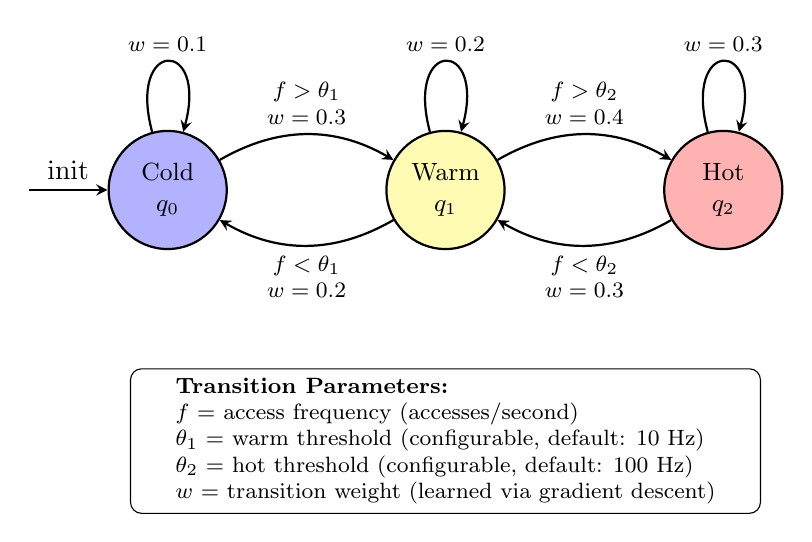
\begin{tikzpicture}[
    node distance=2cm,
    state/.style={circle, draw, thick, minimum size=1.5cm, align=center, font=\small},
    hot/.style={state, fill=red!30},
    warm/.style={state, fill=yellow!30},
    cold/.style={state, fill=blue!30},
    arrow/.style={->, >=stealth, thick},
    label/.style={font=\footnotesize, align=center}
]

% States
\node[cold] (cold) {Cold\\$q_0$};
\node[warm, right=of cold] (warm) {Warm\\$q_1$};
\node[hot, right=of warm] (hot) {Hot\\$q_2$};

% Initial arrow
\draw[arrow] ($(cold.west)+(-1,0)$) -- (cold) node[midway, above] {init};

% Transitions
\draw[arrow, bend left=30] (cold) to node[above, label] {$f > \theta_1$\\$w = 0.3$} (warm);
\draw[arrow, bend left=30] (warm) to node[below, label] {$f < \theta_1$\\$w = 0.2$} (cold);

\draw[arrow, bend left=30] (warm) to node[above, label] {$f > \theta_2$\\$w = 0.4$} (hot);
\draw[arrow, bend left=30] (hot) to node[below, label] {$f < \theta_2$\\$w = 0.3$} (warm);

% Self loops
\draw[arrow] (cold) to[loop above] node[label] {$w = 0.1$} (cold);
\draw[arrow] (warm) to[loop above] node[label] {$w = 0.2$} (warm);
\draw[arrow] (hot) to[loop above] node[label] {$w = 0.3$} (hot);

% Legend
\node[draw, rounded corners, fill=white, below=1.5cm of warm, minimum width=8cm, align=left, font=\footnotesize] (legend) {
    \textbf{Transition Parameters:}\\
    $f$ = access frequency (accesses/second)\\
    $\theta_1$ = warm threshold (configurable, default: 10 Hz)\\
    $\theta_2$ = hot threshold (configurable, default: 100 Hz)\\
    $w$ = transition weight (learned via gradient descent)
};

\end{tikzpicture}
\caption{Weighted Finite Automaton for tensor classification. Transition weights are learned from runtime telemetry.}
\label{fig:wfa}
\end{figure}

\subsection{Data Flow Architecture}

\begin{figure}[htbp]
\centering
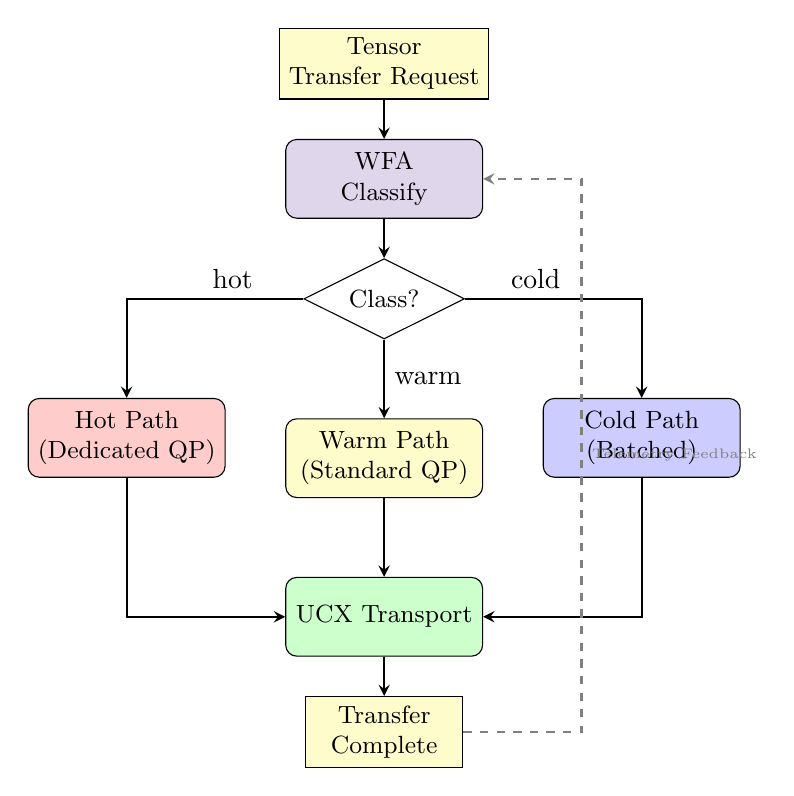
\begin{tikzpicture}[
    node distance=0.5cm and 1cm,
    process/.style={rectangle, draw, rounded corners, minimum width=2.5cm, minimum height=1cm, align=center, font=\small},
    decision/.style={diamond, draw, aspect=2, minimum width=2cm, align=center, font=\small},
    data/.style={rectangle, draw, fill=yellow!20, minimum width=2cm, minimum height=0.6cm, align=center, font=\small},
    arrow/.style={->, >=stealth, thick}
]

% Input
\node[data] (tensor) {Tensor\\Transfer Request};

% Classification
\node[process, fill=wfapurple!20, below=of tensor] (classify) {WFA\\Classify};

% Decision
\node[decision, below=of classify] (check) {Class?};

% Paths
\node[process, fill=red!20, below left=1cm and 1.5cm of check] (hotpath) {Hot Path\\(Dedicated QP)};
\node[process, fill=yellow!20, below=1cm of check] (warmpath) {Warm Path\\(Standard QP)};
\node[process, fill=blue!20, below right=1cm and 1.5cm of check] (coldpath) {Cold Path\\(Batched)};

% UCX
\node[process, fill=green!20, below=1cm of warmpath] (ucx) {UCX Transport};

% Output
\node[data, below=of ucx] (complete) {Transfer\\Complete};

% Arrows
\draw[arrow] (tensor) -- (classify);
\draw[arrow] (classify) -- (check);
\draw[arrow] (check) -| node[pos=0.2, above] {hot} (hotpath);
\draw[arrow] (check) -- node[right] {warm} (warmpath);
\draw[arrow] (check) -| node[pos=0.2, above] {cold} (coldpath);
\draw[arrow] (hotpath) |- (ucx);
\draw[arrow] (warmpath) -- (ucx);
\draw[arrow] (coldpath) |- (ucx);
\draw[arrow] (ucx) -- (complete);

% Telemetry feedback
\draw[arrow, dashed, gray] (complete.east) -- ++(1.5,0) |- (classify.east) node[pos=0.25, right, font=\tiny, align=left] {Telemetry Feedback};

\end{tikzpicture}
\caption{Data flow through the adaptive RDMA middleware showing classification and routing paths.}
\label{fig:dataflow}
\end{figure}

%=============================================================================
\section{Implementation Plan}
%=============================================================================

\subsection{Hardware Testbed}

\begin{table}[htbp]
\centering
\caption{Available hardware resources for implementation and validation}
\label{tab:hardware}
\begin{tabular}{@{}llll@{}}
\toprule
\textbf{System} & \textbf{GPUs} & \textbf{Network} & \textbf{Role} \\
\midrule
Cerberus & 2$\times$ RTX 5090 (64GB total) & 10GbE (iWARP) & Primary inference node \\
Chimera & 3$\times$ RTX 3090 (72GB total) & 10GbE (iWARP) & Training/secondary inference \\
Lab NIC Pool & Mellanox ConnectX-4 IB & 100GbE (upgrade path) & High-bandwidth experiments \\
Intel X710 & -- & 10GbE iWARP & Consumer RDMA validation \\
\bottomrule
\end{tabular}
\end{table}

\subsection{12-Month Timeline}

\begin{figure}[htbp]
\centering
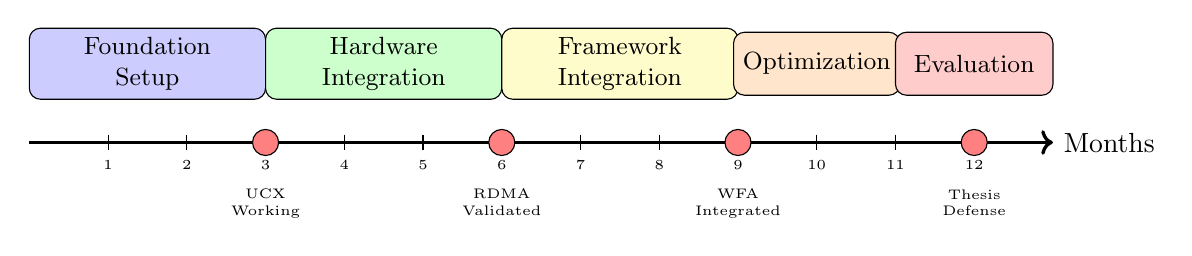
\begin{tikzpicture}[
    node distance=0.3cm,
    phase/.style={rectangle, draw, rounded corners, minimum height=0.8cm, align=center, font=\small},
    milestone/.style={circle, draw, fill=red!50, minimum size=0.3cm}
]

% Timeline
\draw[very thick, ->] (0,0) -- (13,0) node[right] {Months};
\foreach \x in {1,...,12} {
    \draw (\x, 0.1) -- (\x, -0.1) node[below, font=\tiny] {\x};
}

% Phases
\node[phase, fill=blue!20, minimum width=3cm] (p1) at (1.5, 1) {Foundation\\Setup};
\node[phase, fill=green!20, minimum width=3cm] (p2) at (4.5, 1) {Hardware\\Integration};
\node[phase, fill=yellow!20, minimum width=3cm] (p3) at (7.5, 1) {Framework\\Integration};
\node[phase, fill=orange!20, minimum width=2cm] (p4) at (10, 1) {Optimization};
\node[phase, fill=red!20, minimum width=2cm] (p5) at (12, 1) {Evaluation};

% Milestones
\node[milestone] (m1) at (3, 0) {};
\node[below=0.3cm of m1, font=\tiny, align=center] {UCX\\Working};

\node[milestone] (m2) at (6, 0) {};
\node[below=0.3cm of m2, font=\tiny, align=center] {RDMA\\Validated};

\node[milestone] (m3) at (9, 0) {};
\node[below=0.3cm of m3, font=\tiny, align=center] {WFA\\Integrated};

\node[milestone] (m4) at (12, 0) {};
\node[below=0.3cm of m4, font=\tiny, align=center] {Thesis\\Defense};

\end{tikzpicture}
\caption{Implementation timeline with key milestones.}
\label{fig:timeline}
\end{figure}

\subsection{Software Stack}

\begin{lstlisting}[language=Python, caption={Core middleware interface design}]
class AdaptiveRDMAMiddleware:
    def __init__(self, config: MiddlewareConfig):
        self.wfa_classifier = WFAClassifier(config.wfa_params)
        self.telemetry = RuntimeTelemetry()
        self.transport = self._init_transport(config)
        
    def _init_transport(self, config):
        # Automatic transport selection with fallback
        if self._detect_container():
            config.ucx_tls = "^shm,rc,tcp"  # Issue #10055 fix
        
        try:
            return UCXTransport(config)
        except UCXInitError:
            return NCCLFallback(config)
    
    async def transfer_tensor(self, tensor: Tensor, dest: int):
        # WFA classification
        classification = self.wfa_classifier.classify(
            tensor.id, tensor.size, self.telemetry.get_access_pattern(tensor.id)
        )
        
        # Route based on classification
        if classification == TensorClass.HOT:
            return await self.transport.send_priority(tensor, dest)
        elif classification == TensorClass.WARM:
            return await self.transport.send_standard(tensor, dest)
        else:  # COLD
            return await self.transport.send_batched(tensor, dest)
\end{lstlisting}

%=============================================================================
\section{Validation Strategy}
%=============================================================================

\subsection{Simulation with UET-HTSIM}

Before hardware deployment, we will validate the WFA classifier and adaptive routing algorithms using the Ultra Ethernet Consortium's HTSIM simulator:

\begin{enumerate}
    \item Model the 5-node cluster topology (2$\times$5090 + 3$\times$3090)
    \item Generate traffic matrices matching LLM inference patterns:
    \begin{itemize}
        \item Incast (all-reduce gradients)
        \item KV cache scatter (point-to-multipoint)
        \item Activation tensors (point-to-point)
    \end{itemize}
    \item Compare Flow Completion Time (FCT) distributions against baseline
\end{enumerate}

\subsection{Performance Metrics}

\begin{table}[htbp]
\centering
\caption{Target performance improvements}
\label{tab:metrics}
\begin{tabular}{@{}lcc@{}}
\toprule
\textbf{Metric} & \textbf{Baseline} & \textbf{Target} \\
\midrule
Time-To-First-Token (TTFT) & Current vLLM & 30--50\% reduction \\
Training iteration time & NCCL baseline & 20--30\% reduction \\
Cross-NUMA latency (>256KB) & 2500$\mu$s & <500$\mu$s \\
RoCE session stability & 90s before crash & >24h continuous \\
Container deployment time & Manual config & Zero-config \\
\bottomrule
\end{tabular}
\end{table}

\subsection{MoE Training Validation}

Final validation will demonstrate training of a Granite 4 / Mamba 2 style MoE model for RISC-V assembly generation:

\begin{enumerate}
    \item Expert parallelism distributed across Cerberus + Chimera
    \item AllToAll communication for expert routing
    \item Measure expert utilization and communication overhead
    \item Compare training throughput with and without adaptive middleware
\end{enumerate}

%=============================================================================
\section{Expected Contributions}
%=============================================================================

\begin{enumerate}
    \item \textbf{Unified Middleware Framework}: First open-source middleware that enables UCX-based RDMA across NVIDIA, Apple Silicon, and consumer hardware with automatic transport selection and fallback.
    
    \item \textbf{WFA Tensor Classifier}: Novel application of weighted finite automata for runtime classification of ML tensor access patterns, enabling intelligent routing decisions.
    
    \item \textbf{Issue Resolution}: Practical solutions to seven critical GitHub issues blocking distributed ML infrastructure adoption.
    
    \item \textbf{Performance Validation}: Comprehensive benchmarks comparing adaptive RDMA optimization against baseline NCCL/UCX on commodity hardware.
    
    \item \textbf{Open-Source Release}: All code, configurations, and documentation released under permissive license for community adoption.
\end{enumerate}

%=============================================================================
\section{Conclusion}
%=============================================================================

The distributed ML ecosystem's fragmentation across communication standards creates compounding failures that block efficient training of large models on consumer hardware. This proposal presents a systematic approach to addressing these challenges through an adaptive middleware layer that:

\begin{itemize}
    \item Abstracts transport-specific details while preserving RDMA performance
    \item Intelligently classifies tensor access patterns for differential routing
    \item Automatically handles container isolation, NUMA topology, and heterogeneous deployments
    \item Enables unified deployment across NVIDIA, Apple Silicon, and consumer NIC configurations
\end{itemize}

By addressing the seven critical blocking issues identified through comprehensive GitHub analysis, this work will enable researchers and practitioners to leverage RDMA benefits on commodity hardware without the current fragmentation penalty.

%=============================================================================
% References
%=============================================================================

\bibliographystyle{plainnat}
\begin{thebibliography}{99}

\bibitem{ucx2015}
Shamis, P., et al. ``UCX: An Open Source Framework for HPC Network APIs and Beyond.'' \textit{IEEE HOTI}, 2015.

\bibitem{nccl2017}
Jeaugey, S. ``NCCL 2.0.'' \textit{GPU Technology Conference}, 2017.

\bibitem{ndp2017}
Handley, M., et al. ``Re-architecting Datacenter Networks and Stacks for Low Latency and High Performance.'' \textit{ACM SIGCOMM}, 2017.

\bibitem{eqds2022}
Olteanu, A., et al. ``EQDS: An Equivalent Queueing Discipline Scheduler.'' \textit{USENIX NSDI}, 2022.

\bibitem{vllm2023}
Kwon, W., et al. ``Efficient Memory Management for Large Language Model Serving with PagedAttention.'' \textit{ACM SOSP}, 2023.

\bibitem{uec2025}
Ultra Ethernet Consortium. ``UEC 1.0 Specification.'' 2025.

\bibitem{flashattn2022}
Dao, T., et al. ``FlashAttention: Fast and Memory-Efficient Exact Attention.'' \textit{NeurIPS}, 2022.

\end{thebibliography}

\end{document}
